\documentclass{article}
\usepackage{graphicx}
\usepackage{setspace}
\begin{document}
  \title{Basic test}
  \author{Carl Capybara\thanks{A thanks block} \and Walter Wombat}
  \date{March 2018}
  \maketitle
  \begin{abstract}
    A thorough test of basic formatting, layout, and figures

    A reference to section~\ref{formatting} from the abstract.
  \end{abstract}

  \section{Sections}

  \subsection{subsection}

  \subsection*{subsection without counter}

  \subsubsection{subsubsection}

  \paragraph{paragraph}

  Some text.

  \subparagraph{subparagraph}

  Some text.

  \subsection{A HEADING IN ALL CAPS SHOULD BE CONVERTED TO TITLE CASE}


  \section{Text formatting} \label{formatting}

  % A lot of this is from https://en.wikibooks.org/wiki/LaTeX/Text_Formatting

  \subsection{Fonts}

  This is \emph{emph} \\
  This is \textrm{textrm} \\
  This is \textsf{textsf} \\
  This is \textsc{Small Caps} \\
  This is \uppercase{uPpeRcAsE} \\
  This is \textit{textit} \\
  This is \texttt{fixed width} \\
  This is \textbf{textbf} \\
  This is \textmd{textmd} \\
  This is \textlf{textlf} \\
  This is \underline{underline} \\

  \subsection{ulem package}

  \usepackage[normalem]{ulem}
  This is \uline{uline} \\
  This is \sout{sout} \\

  \subsection{Sizing}

  {\tiny tiny} \\
  {\scriptsize scriptsize} \\
  {\footnotesize footnotesize} \\
  {\small small} \\
  {\normalsize normalsize} \\
  {\large large} \\
  {\Large Large} \\
  {\LARGE LARGE} \\
  {\huge huge} \\
  {\Huge Huge} \\

  \subsection{Colors}

  \usepackage{xcolor}

  {black text \color{red}red text}

  \colorbox{red}{\color{white}white text on red background}

  \subsection{Spacing}

  The last two words have a non-breaking~space.

  Before hfill. \hfill After hfill.

  \begin{doublespace}
    This paragraph has \\ double \\ line spacing.
  \end{doublespace}

  \subsection{Quotes}

  To `quote' in LaTeX \\
  To ``quote'' in LaTeX \\
  To ``quote" in LaTeX \\
  To ,,quote'' in LaTeX \\
  ,,German quotation marks`` \\
  <<French quotation marks>> \\
  ``Please press the `x' key.'' \\
  ,,Proszę, naciśnij klawisz <<x>>''.

  \subsection{Super/subscript}

  Some\textsuperscript{superscript} \\
  Some\textsubscript{subscript}

  \subsection{Dashes and hypens}

  Hyphen: daughter-in-law, X-rated\\
  En dash: pages 13--67\\
  Em dash: yes---or no? \\
  Minus sign: $0$, $1$ and $-1$

  \subsection{Ellipsis}

  Not like this ... but like this:\\
  New York, Tokyo, Budapest, \ldots

  \section{Paragraph formatting}

  \subsection{Justification}

  \begin{flushleft}Some text flushed left.\end{flushleft}

  {\raggedright{}Some text ragged right.}

  \begin{flushright}Some text flushed right.\end{flushright}

  {\raggedleft{}Some text ragged left.}

  \begin{center}
    Some text centered.
  \end{center}

  {\centering{}Some text centered.}

  \subsection{Indentation}

  \indent This is indented.

  \subsection{indentfirst package}
  TODO

  \subsection{parskip package}
  TODO

  \subsection{Verbatim}

  \begin{verbatim}
  The verbatim environment
    simply reproduces every
   character you input,
  including all  s p a c e s!
  \end{verbatim}

  \verb+verb command+

  \section{URLs}

  http link: http://link.co.uk/to\#something \\
  https link: https://link.info?param url \\
  link with trailing period: https://example.com. (FIXME: known failure) \\
  this should not make a link: foo.bar \\
  this is a link without leading space: badlatex.http://example.com \\
  this is already a link with href: \href{http://example.com}{example.com} \\
  this is a link without http: \href{example.com}{example.com} \\
  this is already a link with url: \url{http://example.com} \\

  \section{Listings}

  \begin{listing}[step]{first line}
    listing command
  \end{listing}

  \usepackage{listings}
  \begin{lstlisting}[language=Pascal]
  for i:=maxint to 0 do
  begin
  { do nothing }
  end;
  Write('Case insensitive ');
  Write('Pascal keywords.');
  \end{lstlisting}

  \section{Lists}

  \begin{itemize}
    \item An unordered list
    \item Second item
  \end{itemize}

  \begin{enumerate}
    \item An ordered list
    \item Second one.
  \end{enumerate}

  \begin{itemize}
    \item A nested unordered list
    \begin{itemize}
      \item First nested item
      \item Second nested item
    \end{itemize}
    \item Second item
  \end{itemize}

  \subsection{A nested ordered list}
  \begin{enumerate}
    \item First item
    \begin{enumerate}
      \item First nested item
      \item Second nested item
    \end{enumerate}
    \item Second item
  \end{enumerate}

  \section{Tables}
  % https://en.wikibooks.org/wiki/LaTeX/Tables

  \subsection{Basic}

  \begin{tabular}{ l c r }
    1 & 2 & 3 \\
    4 & 5 & 6 \\
    7 & 8 & 9 \\
  \end{tabular}

  \subsection{Vertical lines}

  \begin{tabular}{ l | c | r }
    1 & 2 & 3 \\
    4 & 5 & 6 \\
    7 & 8 & 9 \\
  \end{tabular}

  \subsection{Horizontal lines at top and bottom}

  \begin{tabular}{ l | c | r }
    \hline
    1 & 2 & 3 \\
    4 & 5 & 6 \\
    7 & 8 & 9 \\
    \hline
  \end{tabular}

  \subsection{Lines between every row}

  \begin{center}
    \begin{tabular}{ l | c | r }
      \hline
      1 & 2 & 3 \\ \hline
      4 & 5 & 6 \\ \hline
      7 & 8 & 9 \\
      \hline
    \end{tabular}
  \end{center}

  \begin{tabular}{|r|l|}
    \hline
    7C0 & hexadecimal \\
    3700 & octal \\ \cline{2-2}
    11111000000 & binary \\
    \hline \hline
    1984 & decimal \\
    \hline
  \end{tabular}

  \subsection{Text column with width}

  \begin{center}
    \begin{tabular}{ | l | l | l | p{5cm} |}
      \hline
      Day & Min Temp & Max Temp & Summary \\ \hline
      Monday & 11C & 22C & A clear day with lots of sunshine.
      However, the strong breeze will bring down the temperatures. \\ \hline
      Tuesday & 9C & 19C & Cloudy with rain, across many northern regions. Clear spells
      across most of Scotland and Northern Ireland,
      but rain reaching the far northwest. \\ \hline
      Wednesday & 10C & 21C & Rain will still linger for the morning.
      Conditions will improve by early afternoon and continue
      throughout the evening. \\
      \hline
    \end{tabular}
  \end{center}

  \subsection{Defining multiple columns}

  \begin{tabular}{l*{6}{c}r}
    Team              & P & W & D & L & F  & A & Pts \\
    \hline
    Manchester United & 6 & 4 & 0 & 2 & 10 & 5 & 12  \\
    Celtic            & 6 & 3 & 0 & 3 &  8 & 9 &  9  \\
    Benfica           & 6 & 2 & 1 & 3 &  7 & 8 &  7  \\
    FC Copenhagen     & 6 & 2 & 1 & 3 &  5 & 8 &  7  \\
  \end{tabular}

  \subsection{Rows spanning multiple columns}

  \begin{tabular}{ |l|l| }
    \hline
    \multicolumn{2}{|c|}{Team sheet} \\
    \hline
    GK & Paul Robinson \\
    LB & Lucas Radebe \\
    DC & Michael Duberry \\
    DC & Dominic Matteo \\
    RB & Dider Domi \\
    MC & David Batty \\
    MC & Eirik Bakke \\
    MC & Jody Morris \\
    FW & Jamie McMaster \\
    ST & Alan Smith \\
    ST & Mark Viduka \\
    \hline
  \end{tabular}

  \subsection{Columns spanning multiple rows}
  \usepackage{multirow}

  \begin{tabular}{ |l|l|l| }
    \hline
    \multicolumn{3}{ |c| }{Team sheet} \\
    \hline
    Goalkeeper & GK & Paul Robinson \\ \hline
    \multirow{4}{*}{Defenders} & LB & Lucas Radebe \\
     & DC & Michael Duburry \\
     & DC & Dominic Matteo \\
     & RB & Didier Domi \\ \hline
    \multirow{3}{*}{Midfielders} & MC & David Batty \\
     & MC & Eirik Bakke \\
     & MC & Jody Morris \\ \hline
    Forward & FW & Jamie McMaster \\ \hline
    \multirow{2}{*}{Strikers} & ST & Alan Smith \\
     & ST & Mark Viduka \\
    \hline
  \end{tabular}

  \begin{tabular}{cc|c|c|c|c|l}
    \cline{3-6}
    & & \multicolumn{4}{ c| }{Primes} \\ \cline{3-6}
    & & 2 & 3 & 5 & 7 \\ \cline{1-6}
    \multicolumn{1}{ |c  }{\multirow{2}{*}{Powers} } &
    \multicolumn{1}{ |c| }{504} & 3 & 2 & 0 & 1 &     \\ \cline{2-6}
    \multicolumn{1}{ |c  }{}                        &
    \multicolumn{1}{ |c| }{540} & 2 & 3 & 1 & 0 &     \\ \cline{1-6}
    \multicolumn{1}{ |c  }{\multirow{2}{*}{Powers} } &
    \multicolumn{1}{ |c| }{gcd} & 2 & 2 & 0 & 0 & min \\ \cline{2-6}
    \multicolumn{1}{ |c  }{}                        &
    \multicolumn{1}{ |c| }{lcm} & 3 & 3 & 1 & 1 & max \\ \cline{1-6}
  \end{tabular}

  \begin{tabular}{ r|c|c| }
    \multicolumn{1}{r}{}
     &  \multicolumn{1}{c}{noninteractive}
     & \multicolumn{1}{c}{interactive} \\
    \cline{2-3}
    massively multiple & Library & University \\
    \cline{2-3}
    one-to-one & Book & Tutor \\
    \cline{2-3}
  \end{tabular}

  \subsection{Table with width}

  \begin{tabular*}{0.75\textwidth}{@{\extracolsep{\fill} } | c | c | c | r | }
    \hline
    label 1 & label 2 & label 3 & label 4 \\
    \hline
    item 1  & item 2  & item 3  & item 4  \\
    \hline
  \end{tabular*}

  \subsection{tabularx}

  \usepackage{tabularx}

  \begin{tabularx}{\textwidth}{ |X|X|X|X| }
    \hline
    label 1 & label 2 & label 3 & label 4 \\
    \hline
    item 1  & item 2  & item 3  & item 4  \\
    \hline
  \end{tabularx}

  \subsection{tabulary}

  \usepackage{tabulary}

  \begin{center}
    \begin{tabulary}{0.7\textwidth}{LCL}
      Short sentences      & \#  & Long sentences                                                 \\
      \hline
      This is short.       & 173 & This is much loooooooonger, because there are many more words.  \\
      This is not shorter. & 317 & This is still loooooooonger, because there are many more words. \\
    \end{tabulary}
  \end{center}

  \subsection{Captions and references}

  \begin{table}[h]
    \begin{tabular}{ c c c }
       cell1 & cell2 & cell3 \\
       cell4 & cell5 & cell6 \\
       cell7 & cell8 & cell9
    \end{tabular}
    \caption{Some numbers.}
    \label{table:1}
  \end{table}

  Take a look at some cool data in table \ref{table:1}.

  \begin{table}[h]
    \caption{Caption at the top is put at the bottom.}
    \begin{tabular}{ c c c }
       cell7 & cell8 & cell9
    \end{tabular}
  \end{table}

  \section{Figures}

  \subsection{Plain includeimage}

  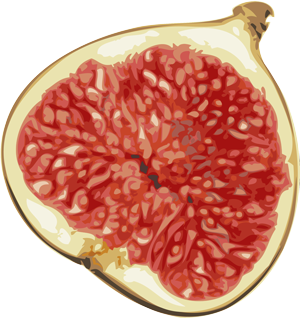
\includegraphics[]{fig.png}

  \subsection{Single image}

  \begin{figure}[h]
    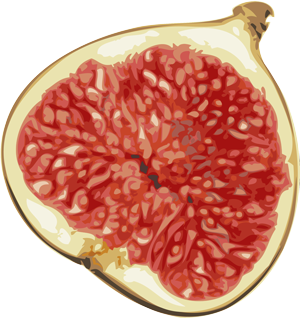
\includegraphics[width=8cm]{fig.png}
    \caption{Fig.}
    \label{fig:fig}
  \end{figure}
  See fig \ref{fig:fig}.

  Ref which doesn't exist \ref{fig:notexist}.

  \subsection{Multiple images}

  \begin{figure}[h]
    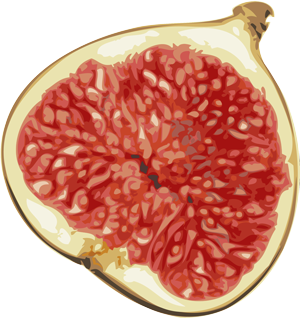
\includegraphics[width=8cm]{fig.png}
    \includegraphics[width=8cm]{fig2.png}
    \caption{Fig.}
    \label{fig:fig}
  \end{figure}
  See fig \ref{fig:fig}.

  \section{Math}

  \subsection{Block}

  \begin{equation}
    e^{i\pi}=-1
    \label{eq:euler}
  \end{equation}
  Equation~\ref{eq:euler} is some good math.

  \subsection{Inline}

  some lovely maths \(x^2 + y^2 = z^2\)

  \section{Footnotes}

  This is some text.\footnote{This is a footnote.} This is some more text.\footnote{And a footnote with a

  second paragraph! And some \emph{formatting}.}

  \section{Citations}

  Refer to \cite{turaga2010affinity} then refer to \cite{vazquez11} but misspell \cite{zlateskiS15_asdf}

  \begin{thebibliography}{}

    \bibitem{turaga2010affinity}
    S.~C. Turaga, J.~F. Murray, V.~Jain, F.~Roth, M.~Helmstaedter, K.~Briggman,
      W.~Denk, and H.~S. Seung.
    \newblock Convolutional networks can learn to generate affinity graphs for
      image segmentation.
    \newblock {\em Neural Comput.}, 22(2):511--538, Feb. 2010.

    \bibitem{vazquez11}
    A.~Vazquez-Reina, M.~Gelbart, D.~Huang, J.~Lichtman, E.~Miller, and H.~Pfister.
    \newblock Segmentation fusion for connectomics.
    \newblock In {\em ICCV}, 2011.

    \bibitem{zlateskiS15}
    A.~Zlateski and H.~S. Seung.
    \newblock Image segmentation by size-dependent single linkage clustering of a
      watershed basin graph.
    \newblock {\em CoRR}, abs/1505.00249, 2015.

  \end{thebibliography}

\end{document}
